% Total economic value decomposition.
% Compile to SVG:  latex tev_tree.tex && dvisvgm --no-fonts tev_tree.dvi -o ../tev_tree.svg
\documentclass[tikz,border=6pt]{standalone}
\usepackage[scaled]{helvet}
\renewcommand{\familydefault}{\sfdefault}
\usetikzlibrary{positioning}
\definecolor{blu}{HTML}{3B6EA8}
\definecolor{accent}{HTML}{2E7D32}
\begin{document}
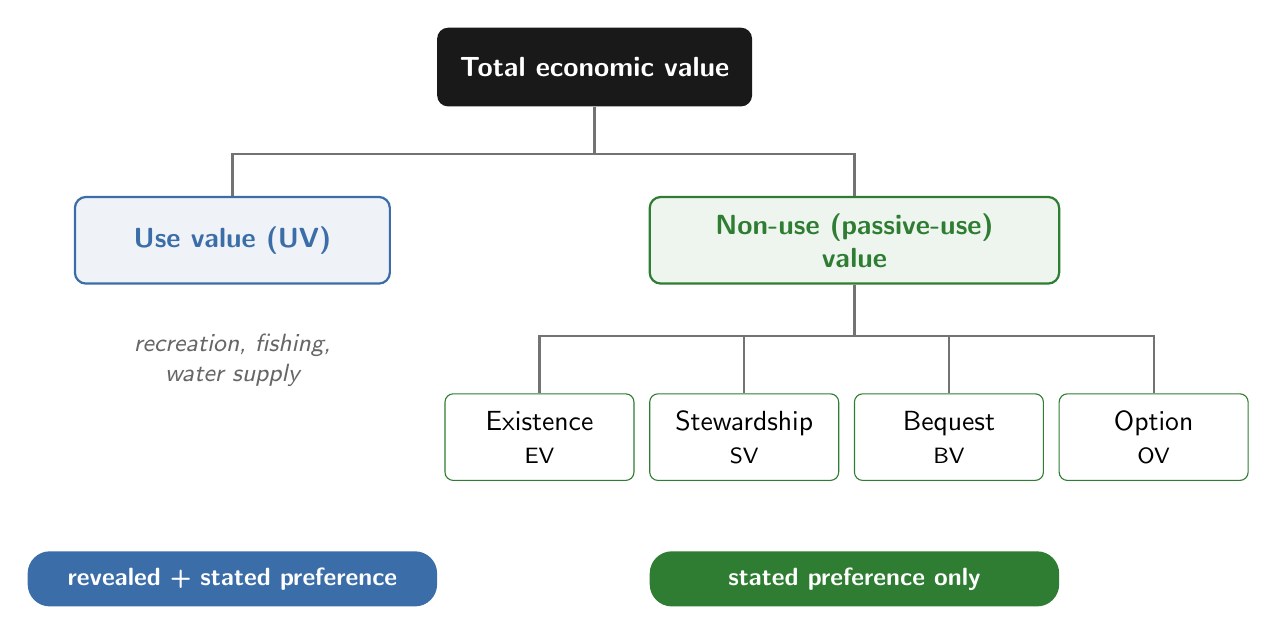
\begin{tikzpicture}[
    edge/.style={draw=black!55, thick, rounded corners=0pt},
    root/.style={fill=black!90, text=white, font=\bfseries, rounded corners=4pt,
                 minimum width=4cm, minimum height=1cm},
    use/.style={draw=blu, fill=blu!8, thick, text=blu, font=\bfseries, rounded corners=4pt,
                minimum width=4cm, minimum height=1.1cm, align=center},
    nonuse/.style={use, draw=accent, fill=accent!8, text=accent, minimum width=5.2cm},
    leaf/.style={draw=accent, fill=white, rounded corners=3pt, minimum width=2.4cm,
                 minimum height=1.1cm, align=center},
    pill/.style={rounded corners=8pt, text=white, font=\small\bfseries,
                 minimum width=5.2cm, minimum height=0.7cm}]
  \node[root] (tev) at (0,0) {Total economic value};
  \node[use]    (uv) at (-4.6,-2.2) {Use value (UV)};
  \node[nonuse] (nu) at ( 3.3,-2.2) {Non-use (passive-use)\\value};
  \node[leaf] (ev) at (-0.7,-4.7) {Existence\\\footnotesize EV};
  \node[leaf] (sv) at ( 1.9,-4.7) {Stewardship\\\footnotesize SV};
  \node[leaf] (bv) at ( 4.5,-4.7) {Bequest\\\footnotesize BV};
  \node[leaf] (ov) at ( 7.1,-4.7) {Option\\\footnotesize OV};
  \draw[edge] (tev.south) -- ++(0,-0.6) -| (uv.north);
  \draw[edge] (tev.south) -- ++(0,-0.6) -| (nu.north);
  \foreach \l in {ev,sv,bv,ov} \draw[edge] (nu.south) -- ++(0,-0.65) -| (\l.north);
  \node[font=\small\itshape, text=black!60, align=center, below=0.5cm of uv]
       {recreation, fishing,\\water supply};
  \node[pill, fill=blu]    at (-4.6,-6.5) {revealed + stated preference};
  \node[pill, fill=accent] at ( 3.3,-6.5) {stated preference only};
\end{tikzpicture}
\end{document}
